\documentclass[11pt]{article}
\usepackage[margin=0.75in]{geometry}
\usepackage{amsmath, amssymb}
\usepackage{graphicx}
\usepackage{verbatim,hyperref}
\usepackage{bm}
%\usepackage{mathrsfs,dsfont,mathtools}
%\usepackage{color}
\usepackage{tikz}
%\usepackage{longtable}
%\newcommand{\unp}[1]{#1^{(0)}}%unperturbed quantities
%\newcommand{\per}[1]{#1^{(1)}}%perturbed quantities
%\newcommand{\sj}[6]{ \begin{Bmatrix}
%     #1 & #2 & #3 \\
%     #4 & #5 & #6	 
%\end{Bmatrix}} %6-j symbol
%\newcommand{\tj}[6]{ \begin{pmatrix}
%     #1 & #2 & #3 \\
%     #4 & #5 & #6	 
%   \end{pmatrix}} %3-j symbol
\allowdisplaybreaks[1]
\numberwithin{equation}{section}
\newcommand{\bt}[1]{\mathbf{#1}}
\newcommand{\wt}[1]{\widetilde{#1}}
\newcommand{\kb}{k_{\rm B}}

\begin{document}

\section{Visibility variance}
\label{sec:visvar}

Suppose we are interested in the intensity within a small patch of sky, and a small frequency slice $\Delta \nu$. Assume these are small enough so that we can approximate the sky to be flat {\em within the patch}. Suppose also that the power per unit frequency is practically constant over a frequency bin $\nu \in (\nu_{\rm 0} - \Delta \nu/2, \nu_{\rm 0} + \Delta \nu/2) \gg 0$, all of which is accessible to our setup. We work with electric fields that have been filtered to keep only these frequencies.

Our experiment operates for a large, but finite time, say ${\cal T}_{\rm obs}$ (say O(yr)). The earth rotates during this period, due to which the patch of sky we observe a) moves on the sky, and b) changes orientation due to field rotation. When working at the level of the electric field, we want to deal with variations solely due to characteristics of the emission ($\nu \sim$ MHz) , rather than this slow rotation ($\nu \sim 10 \ \mu {\rm Hz}$). Hence we bin the data into smaller intervals of duration $\cal T$ (say O(min)), within which we can neglect the earth's rotation. 

Over a time interval $\cal T$, we cannot resolve frequencies that differ by less than $\vert \Delta \nu_{\cal T} \vert = 1/\cal T$. Owing to this, we collapse frequencies between $\nu_0 + (m-1/2)/\cal T$ and $\nu_0 + (m+1/2)/\cal T$ into a discrete mode with frequency $\nu_m \equiv \nu_0 + (m/\cal T)$. We choose the time period $\cal T$ to be long enough so that we can comfortably resolve the frequency range, i.e., $1/{\cal T} \ll \Delta \nu \ll \nu_0$.

\subsection{Incident electric field} 
\label{subsec:incident}

Let the electric field in the region of our setup be $E_\alpha(\bt r, t)$. We write the electric field as a sum over discrete modes as follows
\begin{align}
  {\bt E}(\bt r, t) & = \frac{1}{\sqrt{2 \cal T}} \sum_m  \sum_{\alpha} \int d\hat{\bt n} \ 
  \left[ \wt{E}_\alpha(\hat{\bt n}, \nu_m) {\bt e}_{\alpha} e^{2\pi i \nu_m (\bt r \cdot \hat{\bt n}/c + t)} + \wt{E}^\ast_\alpha(\hat{\bt n}, \nu_m) {\bt e}_{\alpha}^\ast e^{-2\pi i \nu_m (\bt r \cdot \hat{\bt n}/c + t)} \right] \mbox{,}  \label{eq:dft}
\end{align}
where $\hat{\bt n}$ is a direction on the sky, $\alpha$ is a polarization index and $\bt e_{\alpha}$ is a polarization vector. We have explicitly written the negative frequency terms so that the electric field is a real quantity \footnote{We choose the factor of $1/\sqrt{2}$ so that $\vert \wt{E}(\nu_m) \vert^2$ is the one-sided power spectral density, which is divided equally into the positive and negative frequencies.}. The number of values of $m$ is $N = \Delta \nu/\Delta \nu_{\cal T} = {\cal T }\Delta \nu \gg 1$. 

Both the electric field and the mode amplitudes are Gaussian RVs (that take on particular values for each measurement of length $\cal T$); the mode amplitudes satisfy
\begin{align}
   \langle \wt{E}^\ast_{\alpha}(\hat{\bt n}, \nu_m) \wt{E}_\beta(\hat{\bt n}^\prime, \nu_n) \rangle 
   & = \kb T_{\rm sky}(\hat{\bt n}, \nu_m) \delta_{\alpha \beta} \delta_{m n} \delta(\hat{\bt n} - \hat{\bt n}^\prime) 
   \approx \kb T_{\rm sky}(\hat{\bt n}, \nu_0) \delta_{m n} \delta_{\alpha \beta} \delta(\hat{\bt n} - \hat{\bt n}^\prime) \mbox{,} \label{eq:stdevdisc}
\end{align}
where we have normalized the squares of the components in units of energy per unit solid angle (${\rm J} \ {\rm Sr}^{-1}$). The expansion in Eq.~\eqref{eq:dft}, and the sky temperature in Eq.~\eqref{eq:stdevdisc}, are appropriate to use when considering the signal from a diffuse source whose intensity (in ${\rm W} \ {\rm m}^{-2} {\rm Hz}^{-1} {\rm Sr}^{-1}$, or ${\rm Jy} \ {\rm Sr}^{-1}$ with the appropriate scaling) is related to the sky temperature as 
\begin{align}
  I(\hat{\bt n}, \nu) & = \frac{2 \nu^2}{c^2} \kb T_{\rm sky}(\hat{\bt n}, \nu) \mbox{.} \label{eq:intensity}
\end{align}
If we were instead operating with point sources of emission, we would need to work with their emissivity $S$ in units of ${\rm W} \ {\rm m}^{-2} {\rm Hz}^{-1}$ or Jy.

The variance (over a number of independent realizations of the window $\cal T$, say) of the electric field at a given time $t$ is  
\begin{align}
~~~ & \!\!\!\!
  \langle {\bt E}(\bt r, t) \cdot {\bt E}(\bt r, t) \rangle \nonumber \\
  & = 
  \frac{1}{2 \cal T} \sum_{\alpha, \beta} \sum_{m, m^\prime} \int\int d\hat{\bt n} d\hat{\bt n}^\prime
  \left\langle \left[ \wt{E}_\alpha^\ast(\hat{\bt n}, \nu_m) {\bt e}_{\alpha}^\ast e^{-2\pi i \nu_m ({\bt r} \cdot \hat{\bt n}/c + t)} + \wt{E}(\hat{\bt n}, \nu_m) {\bt e}_{\alpha} e^{2\pi i \nu_m ({\bt r} \cdot \hat{\bt n}/c + t)} \right] \cdot \right. \nonumber \\
  & \hspace{126pt} \left. \left[ \wt{E}_\beta(\hat{\bt n}^\prime, \nu_{m^\prime}) {\bt e}_{\beta} e^{2\pi i \nu_{m^\prime} ({\bt r} \cdot \hat{\bt n}^\prime/c + t)} + \wt{E}^\ast(\hat{\bt n}^\prime, \nu_{m^\prime}) {\bt e}_{\beta}^\ast e^{-2\pi i \nu_{m^\prime} ({\bt r} \cdot \hat{\bt n}^\prime/c + t)} \right] \right\rangle \nonumber \\  
  & = \frac{2}{\cal T} \sum_{m} \int d\hat{\bt n} \ \kb T_{\rm sky}(\hat{\bt n}, \nu_m) \nonumber \\
  & \approx \frac{2}{\cal T} N \left[ \int d\hat{\bt n} \ \kb T_{\rm sky}(\hat{\bt n}, \nu_0) \right] 
  = 2 \left[ \int d\hat{\bt n} \ \kb T_{\rm sky}(\hat{\bt n}, \nu_0) \right] \Delta \nu \mbox{.} \label{eq:power}
\end{align}
In going from the first to the second equality, we used Eq.~\eqref{eq:stdevdisc}. The multiplicative factor arises due to the two polarizations. In general, there is a frequency dependent factor multiplying the expansion in Eq.~\eqref{eq:dft} and the result in Eq.~\eqref{eq:power}, but we absorb it into the antennas' response.

\subsection{Antenna response}
\label{subsec:antenna}

The voltage signal at the output of an antenna ${\rm a}_i$, at position $\bt r_i$, is some linear function of the incident electric field, with an additive noise component that originates in the local electronics
\begin{align}
  V({\rm a}_i) & = \mathcal{L}\left[{\bt E}({\bt r}_i)\right] + N({\rm a}_i) \mbox{.} \label{eq:linrealsp}
\end{align}
We decompose the voltage and noise signals into modes in the same manner as the electric field
\begin{align}
  [V/N]({\rm a}_i, t) & = \frac{1}{\sqrt{2 \cal T}} \sum_{m > 0} \left[ [\wt{V}/\wt{N}]({\rm a}_i, \nu_m) e^{2\pi i \nu_m t} + [\wt{V}/\wt{N}]^\ast({\rm a}_i, \nu_m) e^{-2\pi i \nu_m t} \right] \mbox{,} \label{eq:Vdft}
\end{align}
where we use units in which power in the waveforms is $P({\rm a}_i) = \langle V({\rm a}_i)^2 \rangle$. The one-sided power spectral density in the noise is
\begin{align}
  \langle \wt{N}^\ast({\rm a}_i, \nu_m) \wt{N}({\rm a}_j, \nu_n) \rangle & = \kb T_{\rm n}(\nu_m) \delta_{i j} \delta_{m n} \approx \kb T_{\rm n} \delta_{i j} \delta_{m n} \label{eq:noisetemp}
\end{align}
where we have introduced the noise temperature, $T_{\rm n}$.

Since the voltage is a scalar and the electric field is a vector, the linear operation involves a projection (i.e., the antenna is sensitive to one polarization). This is clear if we write out Eq.~\eqref{eq:linrealsp} in the frequency domain by substituting Eq.~\eqref{eq:dft}\footnote{In writing identical beam patterns for all antennas, and assuming that the noise components of each output depend only on the local noise, we are neglecting antenna crosstalk.}:
\begin{align}
  \wt{V}({\rm a}_i, \nu_m) & = \sum_\alpha \int d\hat{\bt n} \ p_{{\rm a}_i \alpha}(\hat{\bt n}) \wt{\mathcal{L}}(\hat{\bt n}, \nu_m)  \wt{E}_\alpha(\hat{\bt n}, \nu_m) e^{ (2\pi i \nu_m/c) {\bt r} \cdot \hat{\bt n}} + \wt{N}({\rm a}_i, \nu_m) \mbox{,} \label{eq:freqtrans}
\end{align}
where $p_{{\rm a}_i \alpha}(\hat{\bt n})$ is a projection onto the antenna's response. The antenna temperature is given by the two-sided output power spectral density (units ${\rm W} \ {\rm Hz}^{-1}$), which is 
\begin{align}
  \kb T_{{\rm a} _i}(\nu_0) & = \frac{1}{\Delta \nu} \langle V({\rm a}_i)^2 \rangle \mbox{.} \label{eq:anttemp}
\end{align}
Given one observation of length $\cal T$, we use the unbiased estimator $\hat{T}_{{\rm a}_i}$, whose definition and expectation value are
\begin{align}
  \kb \hat{T}_{{\rm a}_i}(\nu_0) & = \frac{1}{{\cal T} \Delta \nu} \int_0^{\cal T} dt \ V({\rm a}_i)^2 \mbox{,} \\
  \kb T_{{\rm a}_i}(\nu_0)
  & = \frac{1}{{\cal T} \Delta \nu} \int_0^{\cal T} dt \ \langle V({\rm a}_i)^2 \rangle
  = \frac{1}{\mathcal{T}\Delta{\nu}} \sum_{m} \langle \wt{V}({\rm a}_i, \nu_m) \wt{V}^\ast({\rm a}_i, \nu_m) \rangle \notag \\
  & \approx \sum_{\alpha} \int d\hat{\bt n} \ \vert p_{{\rm a}_i \alpha}(\hat{\bt n}) \vert^2 \vert \wt{\mathcal{L}}(\hat{\bt n}, \nu_0) \vert^2 \kb T_{\rm sky}(\hat{\bt n}, \nu_0) + \kb T_{\rm n} \notag \\
  & = \int d\hat{\bt n} \ \vert \wt{\mathcal{L}}(\hat{\bt n}, \nu_0) \vert^2 \kb T_{\rm sky}(\hat{\bt n}, \nu_0) + \kb T_{\rm n} \mbox{.} \label{eq:antresponse1}
\end{align}
In going from the first to the second line, we used the expansion in Eq.~\eqref{eq:Vdft}. In going from the second to the third line, we substituted Eq.~\eqref{eq:freqtrans}, used the definition of the noise and sky temperatures in Eqs.~\eqref{eq:stdevdisc} and \eqref{eq:noisetemp}, and used the assumption that the sky and system properties don't vary with frequency over the range of interest. In the last line, we used the fact that the projection $p_{{\rm a}_i \alpha}(\hat{\bt n}) = {\bt e}_\alpha(\hat{\bt n}) \cdot {\bt e}_{{\rm a}_i}(\hat{\bt n})$ to replace the summation over the polarizations with unity. The voltage transfer function is related to the effective area, $A(\hat{\bt n}, \nu_0)$, by
\begin{align}
  \vert \wt{\mathcal{L}}(\hat{\bt n}, \nu_0) \vert^2 = \frac{\nu_0^2}{c^2} A(\hat{\bt n}, \nu_0) \mbox{,}
\end{align}
Let us assume that to the lowest approximation, the sky temperature is uniform and equals $T_{\rm sky}$. In that case, using a fundamental identity of antenna theory, we can do the angular integral over the beam in Eq.~\eqref{eq:antresponse1} and obtain\footnote{If the emission in the patch were instead dominated by a point source, we have $T_{{\rm a}_i} = \frac{1}{2} A(\hat{\bt n}_0, \nu_0) S + T_{\rm n}$, where $S$ is the point source's flux in ${\rm W} {\rm m}^{-2} {\rm Hz}^{-1}$, or Jy.}
\begin{align}
  T_{{\rm a}_i} & = T_{\rm sky} + T_{\rm n} \mbox{.} \label{eq:anttemp2}
\end{align}
It is also useful to define the following autocorrelation function of the antenna's output
\begin{align}
  A_{{\rm a}_i}(\nu_0, \tau) & = \frac{1}{\Delta\nu} \langle V({\rm a}_i, t) V({\rm a}_i, t + \tau) \rangle \mbox{.} \label{eq:autocorrdef}
\end{align}
It is related to the frequency components by a Fourier transform (the Weiner-Khinchin theorem). Under our set of assumptions, it evaluates to
\begin{align}
~~~ & \!\!\!\!
  A_{{\rm a}_i}(\nu_0, \tau) \nonumber \\
  & = \frac{1}{2 \mathcal{T} \Delta\nu } \sum_{m, m^\prime} \left\langle \left[ \wt{V}({\rm a}_i, \nu_m) e^{2\pi i \nu_m t} + \wt{V}^\ast({\rm a}_i, \nu_m) e^{-2\pi i \nu_m t} \right] \left[ \wt{V}({\rm a}_i, \nu_{m^\prime}) e^{2\pi i \nu_{m^\prime} (t + \tau)} + \wt{V}^\ast({\rm a}_i, \nu_{m^\prime}) e^{-2\pi i \nu_{m^\prime} (t + \tau)} \right] \right\rangle \notag \\
  & = \frac{1}{\mathcal{T} \Delta\nu} \sum_{m} \left\langle \wt{V}({\rm a}_i, \nu_m) \wt{V}^\ast({\rm a}_i, \nu_m) \right\rangle \cos{(2\pi \nu_m \tau)} \notag \\
  & \approx \left[ \frac{1}{\mathcal{T} \Delta\nu} \sum_{m} \cos{(2\pi \nu_m \tau)} \right] \kb T_{{\rm a}_i}(\nu_0)   \notag \\
  & = \left[ \frac{1}{\mathcal{T} \Delta\nu} \frac{ \sin{(\pi \tau \Delta\nu)} }{ \sin{(\pi \tau/\mathcal{T})} } \right] \cos{(2 \pi \nu_0 \tau)} \ \kb T_{{\rm a}_i}(\nu_0) \mbox{,} \label{eq:autocorr}
\end{align}
where in going from the second to the third line, we approximated the slowly varying signal term by its value at the band-center. When $t > \mathcal{T} - \tau$, the shifted voltage should be considered as living in a periodic extension of the observed window. Note that the autocorrelation is an even function.

\subsection{Visibilities}
\label{sec:visibilities}

\begin{figure}[htp]
  \centering
  \includegraphics[width=8cm]{schematic}
\caption{\label{fig:schematic} Schematic figure of readout setup. The notation is explained in the body of the text.}
\end{figure}

In this section we describe how we compute the complex visibility from measured voltages, which will help us analyze the former's variance. 

Figure \ref{fig:schematic} shows a schematic of our setup and the elements involved in post-processing. We assume that the antennas are in tracking mode, i.e., their beam centers alway point toward our patch's center as the earth rotates. We also assume that either the primary beam is azimuthally symmetric, or that the antennas are equatorially mounted. A real setup would have a non-linear element in order to mix down the signal to more manageable frequencies. We neglect this aspect in our analysis.

A single baseline consists of a pair of identical antennas at two different locations, say $\bt r_i$ and $\bt r_j$ with a separation vector $\rm r_{ij} = {\bt r}_i - {\bt r}_j$. If our patch's center is towards the direction $\hat{\bt n}_0$, the geometric delay between arrival times of a wavefront emitted from the center is $\tau_0 = - {\bt r}_{ij} \cdot \hat{\bt n}_0/c$. The setup introduces an additional time-delay to cancel this out, so that signals from the patch's center are in phase at the readout. The setup in Fig.~\ref{fig:schematic} is a complex correlator, i.e., it includes an additional element that introduces a phase-shift in one of the signals before sending it to the second multiplier.

The first multiplier measures the cross-power per unit frequency (in units of ${\rm W} \ {\rm Hz}^{-1}$, or ${\rm J} \ {\rm beam}^{-1}$), of the signals after applying a delay. We call this $C_{ij}$, for reasons that will become obvious later.
\begin{align}
  C_{ij}(\nu_0) & = \frac{1}{\Delta \nu} \langle V({\rm a}_i, t) V({\rm a}_j, t - \tau_0) \rangle \mbox{.}
\end{align}
Over one observation window of length $\cal T$ during which we measure the voltages, we use the estimator
\begin{align}
 \hat{C}_{ij}(\nu_0) = \frac{1}{{\cal T} \Delta\nu} \int_0^{\cal T} dt \ V(\rm a_i, t) V(\rm a_j, t - \tau_0) \mbox{.} \label{eq:visibility} %\qquad \langle \hat{\mathcal{C}}_{ij} \rangle = \mathcal{C}_{ij} \mbox{.} 
\end{align}
We evaluate this by substituting Eqs.~\eqref{eq:Vdft} and \eqref{eq:freqtrans} and following steps similar to those that led to Eq.~\eqref{eq:antresponse1}.
\begin{align}
~~~ & \!\!\!\!
  \langle \hat{C}_{ij}(\nu_0) \rangle \nonumber \\
  & = \frac{1}{{\cal T} \Delta\nu} \int_0^{\cal T} dt \ \langle V(\rm a_i, t) V(\rm a_j, t - \tau_0) \rangle \notag \\
%  
  & = \frac{1}{2 {\cal T}^2 \Delta\nu} \sum_{m, m^\prime} \int_0^{\cal T} dt \ \left\langle \left[ \wt{V}({\rm a_i}, \nu_m) e^{2\pi i \nu_m t} + \wt{V}^\ast({\rm a_i}, \nu_m) e^{-2\pi i \nu_m t} \right] \times \right. \notag \\ 
  & \hspace{114pt} \left. \left[ \wt{V}({\rm a_j}, \nu_{m^\prime}) e^{2\pi i \nu_{m^\prime} (t - \tau_0)} + \wt{V}^\ast({\rm a_j}, \nu_{m^\prime}) e^{-2\pi i \nu_{m^\prime} (t - \tau_0)} \right] \right\rangle \notag \\
%  
  & = \frac{1}{2 {\cal T}^2 \Delta\nu} \sum_{\alpha, \beta} \sum_{m, m^\prime} \int_0^{\cal T} dt \int \int d\hat{\bt n} d\hat{\bt n}^\prime \notag \\
  & \hspace{20pt} \left\langle \left[ p_{{\rm a}_i \alpha}(\hat{\bt n})  \wt{\mathcal{L}}(\hat{\bt n}, \nu_{m}) \hat{E}_\alpha(\hat{\bt n}, \nu_{m}) e^{2\pi i \nu_{m} (\bt r_i \cdot \hat{\bt n}/c + t)} + p_{{\rm a}_i \alpha}^\ast(\hat{\bt n}) \wt{\mathcal{L}}^\ast(\hat{\bt n}, \nu_{m}) \hat{E}^\ast_\alpha(\hat{\bt n}, \nu_{m}) e^{-2\pi i \nu_{m} (\bt r_i \cdot \hat{\bt n}/c + t)} \right] \times \right. \notag \\ 
  & \hspace{25pt} \left. \left[ p_{{\rm a}_j \beta}(\hat{\bt n}^\prime) \wt{\mathcal{L}}(\hat{\bt n}^\prime, \nu_{m^\prime}) \hat{E}_\beta(\hat{\bt n}^\prime, \nu_{m^\prime}) e^{2\pi i \nu_{m^\prime} (\bt r_j \cdot \hat{\bt n}^\prime/c + t - \tau_0)} + p_{{\rm a}_j \beta}^\ast(\hat{\bt n}^\prime) \wt{\mathcal{L}}^\ast(\hat{\bt n}^\prime, \nu_{m^\prime}) \hat{E}^\ast_\beta(\hat{\bt n}^\prime, \nu_{m^\prime})  e^{-2\pi i \nu_{m^\prime} (\bt r_j \cdot \hat{\bt n}^\prime/c + t - \tau_0)} \right] \right\rangle  \notag \\
%  
  & = \frac{1}{{\cal T} \Delta\nu} \sum_{\alpha} \sum_{m} \int d\hat{\bt n} \ \vert p_{{\rm a}_i \alpha}(\hat{\bt n}) \vert^2 \vert \wt{\mathcal{L}}(\hat{\bt n}, \nu_{m}) \vert^2 \kb T_{\rm sky}(\hat{\bt n}, \nu_m)  \cos{\left[ 2\pi \nu_{m} \bt r_{ij} \cdot (\hat{\bt n} - \hat{\bt n}_0)/c \right]} \notag \\
%  
  & \approx \int d\hat{\bt n} \ \vert \wt{\mathcal{L}}(\hat{\bt n}, \nu_{0}) \vert^2 \kb T_{\rm sky}(\hat{\bt n}, \nu_0) \cos{\left[ 2\pi \nu_{0} \bt r_{ij} \cdot (\hat{\bt n} - \hat{\bt n}_0)/c \right]} = \frac12 \int d\hat{\bt n} \ A(\hat{\bt n}, \nu_0) I(\hat{\bt n}, \nu_0)  \cos{\left[ 2\pi \nu_{0} \bt r_{ij} \cdot (\hat{\bt n} - \hat{\bt n}_0)/c \right]} \mbox{,} \label{eq:visibilitydef}
\end{align}
where $\bt r_{ij} = \bt r_i - \bt r_j$ denotes the separation of the antennas, we have assumed that the noise in the two antennas is uncorrelated, and that they have identical polarization behaviour. Due to the extra time-delay by $\tau_0$, the argument of the cosine in the fourth line oscillates slowly over the range of frequencies, and we replace it with its value at the band-center in the final line\footnote{In general, the final answer is modulated by a sinc function in the same manner as Eq.~\eqref{eq:autocorr}. Due to the smallness of the argument, it is acceptable to neglect the variation with frequency. We expand on this in Sec.~\ref{subsec:reconstruction}. \label{fn:bw}}.

We now assume that the antenna beam is small enough in order to make the flat sky approximation over the entire range of angles that fall within. This is important to justify the Fourier transform relation between the visibility and the intensity. To relax this assumption, we must instead use the techniques described in Shaw, R. et. al., (2014).
%\footnote{We assume that we are probing intensity structure {\em within} the beam during each time-bin of length $\cal T$. We will then use multiple time bins to improve errors, and not to map out other regions of a Fourier mode that is larger than the beam, i.e., we are not doing Arecibo-style intensity mapping.}

Under this approximation, Eq.~\eqref{eq:visibilitydef} becomes 
\begin{align}
  \langle \hat{C}_{ij}(\nu_0) \rangle & = \frac12 \int d \bm{\sigma} A(\bm \sigma, \nu_0) I(\bm \sigma, \nu_m)  \cos{\left[ 2\pi \nu_{0} \bt r_{ij} \cdot \bm \sigma/c \right]} \mbox{,} \label{eq:visibilityflat}
\end{align}
where $\bm \sigma = \hat{\bt n} - \hat{\bt n}_0$ lives on a Euclidean plane.

The additional phase-shifter in the output from antenna ${\rm a}_i$ in Fig.~\ref{fig:schematic} converts the signal $V({\rm a}_i)$ to a new signal $V^{\rm S}({\rm a}_i)$, defined as
\begin{align}
    V^{\rm S}({\rm a}_i, t) & = \frac{1}{\sqrt{2 \cal T}} \sum_{m > 0} \left[ \wt{V}({\rm a}_i, \nu_m) e^{i(2\pi  \nu_m t - \pi/2)} + \wt{V}^\ast({\rm a}_i, \nu_m) e^{-i(2\pi \nu_m t - \pi/2)} \right] \\ 
    & = \frac{1}{\sqrt{2 \cal T}} \sum_{m > 0} i \left[ - \wt{V}({\rm a}_i, \nu_m) e^{2\pi i \nu_m t} + \wt{V}^\ast({\rm a}_i, \nu_m) e^{- 2\pi i \nu_m t} \right] \mbox{,} \label{eq:VSdef}
\end{align}
where the frequency components are identical to those in Eq.~\eqref{eq:Vdft}. Note that $V^{\rm S}({\rm a}_i)$ is also a real waveform -- this is the so-called {\em quadrature component}. 

The second multiplier measures a quantity $S_{ij}$, which is defined as
\begin{align}
  S_{ij}(\nu_0) & = \frac{1}{\Delta \nu} \langle V^{\rm S}({\rm a}_i, t) V({\rm a}_j, t - \tau_0) \rangle \mbox{.}
\end{align}
The estimator $\hat{S}_{ij}$ is analogous to the definition for $\hat{C}_{ij}$. We obtain its expectation value by following similar steps as those that led to Eqs.~\eqref{eq:visibilitydef} and \eqref{eq:visibilityflat}:
\begin{align}
  \langle \hat{S}_{ij}(\nu_0) \rangle & = \frac12 \int d \bm{\sigma} A(\bm \sigma, \nu_0) I(\bm \sigma, \nu_0)  \sin{\left[ 2\pi \nu_{0} \bt r_{ij} \cdot \bm \sigma/c \right]} \mbox{.} \label{eq:visibilitysineflat}
\end{align}
The complex visibility, $\mathcal{V}_{ij}$, is defined by
\begin{align}
  \mathcal{V}_{ij}(\nu_0) & = C_{ij}(\nu_0) + i S_{ij}(\nu_0) \mbox{.}
\end{align}

Now we proceed to calculate the variance of the estimators $\hat{C}_{ij}$ and $\hat{S}_{ij}$. The consideration of the antenna crosstalk etc require us to place them at some reasonable separation compared to the wavelength, hence we can assume that the fields at widely separated points are weakly correlated. As a consequence, we throw away any correlation between the voltages at different antennas while computing variances.
\begin{align}
  \langle \hat{C}_{ij}(\nu_0) \hat{C}_{ij}(\nu_0) \rangle & = \frac{1}{{\cal T}^2 \Delta \nu^2} \int_0^{\cal T} \int_0^{\cal T} dt dt^\prime \ \langle V({\rm a}_i, t) V({\rm a}_j, t - \tau_0) V({\rm a}_i, t^\prime) V({\rm a}_j, t^\prime - \tau_0) \rangle \notag \\
  & \approx \frac{1}{{\cal T}^2 \Delta \nu^2} \int_0^{\cal T} \int_0^{\cal T} dt dt^\prime \ \langle V({\rm a}_i, t) V({\rm a}_i, t^\prime) \rangle \langle V({\rm a}_j, t - \tau_0)  V({\rm a}_j, t^\prime - \tau_0) \rangle \notag \\
  & = \frac{1}{{\cal T}^2} \int_0^{\cal T} \int_0^{\cal T} dt dt^\prime \ A_{{\rm a}_i}(\nu_0, t^\prime - t) A_{{\rm a}_j}(\nu_0, t^\prime - t) \mbox{.}
\end{align}
In going from the first to the second line, we use Wick's theorem, and retain only terms involving correlations between identical antennas' outputs. In the third line, we use the definition of the autocorrelation function in Eq.~\eqref{eq:autocorrdef}. 

We simplify the result by performing a change of variables to $a = t + t^\prime$ and $b = t^\prime - t$:
\begin{align}
  \langle \hat{C}_{ij}(\nu_0) \hat{C}_{ij}(\nu_0) \rangle & = \frac{1}{{\cal T}^2} \left[ \frac12 \int_0^{\cal T} da \int_{-a}^{a} db \ A_{{\rm a}_i}(\nu_0, b) A_{{\rm a}_j}(\nu_0, b) + \frac12 \int_{\cal T}^{2 \cal T} da \int_{- 2{\cal T} + a}^{2{\cal T} - a} db \ A_{{\rm a}_i}(\nu_0, b) A_{{\rm a}_j}(\nu_0, b) \right] \notag \\
  & = \frac{1}{{\cal T}^2} \int_0^{\cal T} da \int_{-a}^{a} db \ A_{{\rm a}_i}(\nu_0, b) A_{{\rm a}_j}(\nu_0, b) \notag \\
  & = \frac{2}{{\cal T}^2} \int_0^{\cal T} da \int_{0}^{a} db \ A_{{\rm a}_i}(\nu_0, b) A_{{\rm a}_j}(\nu_0, b) \notag \\
  & = \frac{2}{{\cal T}^2} \int_{0}^{\cal T} db \ ({\cal T} - b) A_{{\rm a}_i}(\nu_0, b) A_{{\rm a}_j}(\nu_0, b) \mbox{.}
\end{align}
We substitute the autocorrelation function from Eq.~\eqref{eq:autocorr} and assume the same antenna temperature for both antennas to get
\begin{align}
  \langle \hat{C}_{ij}(\nu_0) \hat{C}_{ij}(\nu_0) \rangle & = \frac{2 (\kb T_{{\rm a}_i}(\nu_0))^2}{{\cal T}^4 (\Delta\nu)^2} \int_{0}^{\cal T} db \ ({\cal T} - b) \left[ \frac{ \sin{(\pi b \Delta\nu)} }{ \sin{(\pi b/\mathcal{T})} } \right]^2 \cos^2{(2 \pi \nu_0 b)} \notag \\
  & = \frac{2 (\kb T_{{\rm a}_i}(\nu_0))^2}{{\cal T}^2 (\Delta\nu)^2} \int_{0}^{1} dx \ (1 - x) \left[ \frac{ \sin{(\pi x {\cal T} \Delta\nu )} }{ \sin{(\pi x)} } \right]^2 \cos^2{(2 \pi \nu_0 {\cal T} x)} \notag \\
  & \approx \frac{(\kb T_{{\rm a}_i}(\nu_0))^2}{N^2} \int_{0}^{1} dx \ (1 - x) \left[ \frac{ \sin{(\pi x N )} }{ \sin{(\pi x)} } \right]^2 \mbox{.}
\end{align}
The ratio of the sine functions approaches $N^2$ near $x \simeq 0$, and dies out beyond $x \simeq 1/N = 1/({\cal T} \Delta \nu)$. In replacing the cosine-squared term by its average value, we have used that $\Delta \nu \ll \nu_0$. The integral evaluates to $N/2$, owing to which we have
\begin{align}
  \langle \hat{C}_{ij}(\nu_0) \hat{C}_{ij}(\nu_0) \rangle & \approx \frac{(\kb T_{{\rm a}_i}(\nu_0))^2}{2 N} = \frac{(\kb T_{{\rm a}_i}(\nu_0))^2}{2 {\cal T} \Delta \nu} \mbox{.}
\end{align}
By going through these steps, we can also verify that $\langle \hat{S}_{ij}(\nu_0) \hat{S}_{ij}(\nu_0) \rangle \approx (\kb T_{{\rm a}_i}(\nu_0))^2/(2 {\cal T} \Delta \nu)$ and $\langle \hat{C}_{ij}(\nu_0) \hat{S}_{ij}(\nu_0) \rangle = 0$.

\subsection{Reconstructing the sky}
\label{subsec:reconstruction}

In this section, we deal with the reconstruction of the sky intensity from the measured visibilities. 

\subsubsection{Single baseline}
\label{subsubsec:singlebl}

To sum up the previous section's results, the estimator for the visibility and its characteristics are
\begin{align}
  \hat{\cal V}_{ij}(\nu_0)  = \hat{C}_{ij}(\nu_0) + i \hat{S}_{ij}(\nu_0) & = \frac{1}{{\cal T}\Delta \nu} \int_0^{\cal T} dt \left[ V({\rm a}_i, t) + i V^{\rm S}({\rm a}_i, t) \right] V({\rm a}_j, t - \tau_0) \mbox{,} \label{eq:visibilityest} \\
  \langle \hat{\cal V}_{ij}(\nu_0) \rangle & = \frac12 \int d \bm{\sigma} A(\bm \sigma, \nu_0) I(\bm \sigma, \nu_0)  e^{ 2\pi i \nu_{0} \bt r_{ij} \cdot \bm \sigma/c } \mbox{,} \label{eq:visibilitymean} \\
  \langle \hat{\cal V}_{ij}^\ast(\nu_0) \hat{\cal V}_{ij}(\nu_0) \rangle & = \frac{( k_{\rm B} T_{{\rm a}_i}(\nu_0) )^2}{{\cal T} \Delta \nu} \mbox{,} \qquad {\rm and} \qquad \langle {\rm Re}(\hat{\cal V}_{ij}(\nu_0)) {\rm Im}(\hat{\cal V}_{ij}(\nu_0)) \rangle = 0 \mbox{.} \label{eq:visibilityvar}
\end{align}
It is useful to write the right-hand side of Eq.~\eqref{eq:visibilitymean} in terms of $l$ and $m$ coordinates, which are Cartesian coordinates on the tangent plane to the celestial sphere at $\hat{\bm n}_0$. These coordinates are defined such that for small angles, the solid angle is $d\Omega = d \bm{\sigma} = dl dm$.
\begin{align}
  \langle \hat{\cal V}_{ij}(\nu_0) \rangle & = \frac12 \int dl dm \ A(l, m, \nu_0) I(l, m, \nu_0)  e^{ 2\pi i (u l + v m)} \\
  & = \frac{A_0}{2} \int dl dm \ {\cal A}(l, m, \nu_0) I(l, m, \nu_0)  e^{ 2\pi i (u l + v m)} \\
  & \approx \frac{A_0}{2 \Delta \nu} \int_{\nu_0 - \Delta \nu/2}^{\nu_0 + \Delta \nu/2} d\nu \int dl dm \ {\cal A}(l, m) I(l, m, \nu) e^{ 2\pi i (u l + v m)} \mbox{.} \label{eq:visibilityscaleda}
\end{align}
where $u$ and $v$ are projections of the antenna separation (in units of the wavelength at band-center) onto the tangent plane at $\hat{\bm n}_0$, $A_0$ is the effective area at the beam center, and ${\cal A}$ is the scaled beam normalized to unity at the center. In Eq.~\eqref{eq:visibilityscaleda}, we have neglected the beam's variation with frequency over the band $\Delta \nu$, and assumed that the measurement is an average over the band. 

We write the visibility as a function of the baseline, and express the mean as a convolution integral according to
\begin{align}
  \langle \hat{\cal V}(u, v, \nu_0) \rangle & = \frac{A_0}{2 \Delta \nu} \int_{\nu_0 - \Delta \nu/2}^{\nu_0 + \Delta \nu/2} d\nu \ \wt{{\cal A} I(\nu) }(u, v) = \frac{A_0}{2 \Delta \nu} \int_{\nu_0 - \Delta \nu/2}^{\nu_0 + \Delta \nu/2} d\nu du^\prime dv^\prime \wt{\cal A}(u^\prime, v^\prime) \wt{I}(u - u^\prime, v - v^\prime, \nu) \mbox{.} \label{eq:vspatialft}
\end{align}
The tilde denotes a spatial Fourier transform \footnote{The $\wt{I}(u, v, \nu)$ in Eq.~\eqref{eq:vspatialft} corresponds to $V(u,v,\theta_\nu)$ in the notation in the macrophysics paper.}, and we are still using the flat sky approximation. Suppose the scaled beam takes a two-dimensional Sinc shape, with the first zeros along both axes at $\pm \Delta l/2$, and $\pm \Delta m/2$, i.e.,
\begin{align}
  {\cal A}(l, m) & \approx \frac{\sin{(2\pi l/\Delta l)}}{2\pi l/\Delta l} \frac{\sin{(2\pi m/\Delta m)}}{2\pi m/\Delta m} \mbox{,} \\
  \wt{\cal A}(u, v) & = \int dl \frac{\sin{(2\pi l/\Delta l)}}{2\pi l/\Delta l} e^{ 2\pi i u l} \int dm \frac{\sin{(2\pi m/\Delta m)}}{2\pi m/\Delta m} e^{ 2\pi i v m} = \frac{\Delta l \Delta m}{4} {\rm Rect}\left( \frac{u \Delta l}{2} \right) {\rm Rect}\left( \frac{v \Delta m}{2} \right) \mbox{,} \label{eq:sincft}
\end{align}
where Rect evaluates to unity when its argument is between $-1/2$ and $1/2$, and zero otherwise. Suppose we define the solid angle of the beam by the integral of the scaled profile, i.e.,
\begin{align}
  \Delta \Omega_{\rm beam} & = \int dl dm \ {\cal A}(l, m) = \frac{\Delta l \Delta m}{4} \mbox{.}
\end{align}
Technically, this solid angle is constrained by the identity that led to Eq.~\eqref{eq:anttemp2}, but let us neglect that for now. In this case, we can use Eq.~\eqref{eq:sincft} to write Eq.~\eqref{eq:vspatialft} as
\begin{align}
  \langle \hat{\cal V}(u, v, \nu_0) \rangle & = \frac{A_0 \Delta \Omega_{\rm beam}}{2 \Delta \nu} \int_{\nu_0 - \Delta \nu/2}^{\nu_0 + \Delta \nu/2} d\nu \int_{1/\Delta \Omega_{\rm beam},(u,v)} du^\prime dv^\prime \ \wt{I}(u^\prime, v^\prime, \nu) \\
  & = \frac{A_0 \Delta \Omega_{\rm beam}}{2 \Delta \nu} \int_{\nu_0 - \Delta \nu/2}^{\nu_0 + \Delta \nu/2} d\nu \int_{1/\Delta \Omega_{\rm beam},(u,v)} du^\prime dv^\prime \ \wt{I}(u^\prime, v^\prime, \nu) \mbox{,} \label{eq:visdiscretize}
\end{align}
where the subscript on the angular integral indicates that it is over a cell of area $1/\Delta \Omega_{\rm beam}$ centered on $(u,v)$. 

By inspecting Eq.~\eqref{eq:visdiscretize}, we obtain the following fundamental result: {\em the visibility estimator from a single baseline in a single band of width $\Delta \nu$ measures the spatially Fourier-transformed intensity field, $\wt{I}(u^\prime, v^\prime, \nu)$, averaged over a cell of size $1/\Delta \Omega_{\rm beam}$ in the u-v plane, and $\Delta \nu$ in the frequency direction.} The relevant region is illustrated in Fig.~\ref{fig:singlecell}.

\begin{figure}[t]
  \centering
  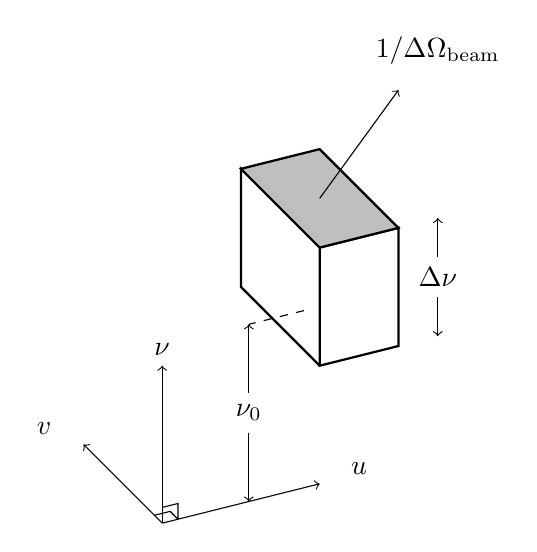
\begin{tikzpicture}
    \draw[->] (0,0) -- (2,0.5);
    \node at (2.5,0.7) {$u$};
    \draw[->] (0,0) -- (-1,1);
    \node at (-1.5,1.2) {$v$};    
    \draw[->] (0,0) -- (0,2);
    \node at (0,2.2) {$\nu$};    
    \draw (0.2,0.05) -- (0.1,0.15) -- (-0.1,0.1);
    \draw (0.2,0.05) -- (0.2,0.25) -- (0,0.2);
%  
    \draw[thick] (2,2) -- (3,2.25) -- (3,3.75) -- (2,3.5) -- cycle;
    \draw[thick] (2,2) -- (1,3) -- (1,4.5) -- (2,3.5);
    \draw[thick, fill=gray!50] (2,3.5) -- (3,3.75) -- (2,4.75) -- (1,4.5) -- cycle;
%
    \draw[<-] (3.5, 2.375) -- (3.5, 2.875);
    \draw[<-] (3.5, 3.875) -- (3.5, 3.375);
    \node at (3.5, 3.125) {$\Delta \nu$};
%
    \draw[dashed] (1.8, 2.70) -- (1.1,2.525);
    \draw[<-] (1.1,2.525) -- (1.1,1.650);
    \draw[->] (1.1,1.150) -- (1.1,0.275);
    \node at (1.1, 1.40) {$\nu_0$};
%
    \draw[->] (2,4.125) -- (3,5.5);
    \node at (3.5,6) {$1/\Delta \Omega_{\rm beam}$};
  \end{tikzpicture}
  \caption{\label{fig:singlecell} Illustration of region in the space of $u$, $v$, and frequency $\nu$, that is accessed by the visibility estimator from a single baseline in a single band of width $\Delta \nu$ about some mean frequency, $\nu_0$. The estimator's mean is the average value in this cell.}
\end{figure}

\subsubsection{Putting together multiple baselines and reconstructing the sky}
\label{subsubsec:multiplebl}

Suppose we are computing the visibility in a cell such as that in Fig.~\ref{fig:singlecell}. In a given frequency band, if we have multiple baselines whose $u$ and $v$ fall within the cell, the variance in our estimator falls by a factor of the number of baselines in the cell. Thus the new variance in the visibility estimator is
\begin{align}
  \langle \hat{\cal V}(u, v, \nu_0)^\ast \hat{\cal V}(u, v, \nu_0) \rangle & = \frac{( k_{\rm B} T_{{\rm a}_i}(\nu_0) )^2}{{\cal T} \Delta \nu} \frac{\Delta \Omega_{\rm beam}}{n(u, v)} \mbox{,} \label{eq:visibilitymult}
\end{align}
where $n(u, v)$ is the number of baselines per unit area in the u-v plane. The presence of multiple baselines also allows us to access multiple cells in the u-v plane in one shot in a single time-bin of length $\cal T$ (we can also access multiple cells by letting the earth's rotation do our job for us).

Until now, we have been thinking of electric fields and voltages within a single band. Suppose now that we measure different bands, so that we can also access multiple cells along the $\nu$ axis in Fig.~\ref{fig:singlecell}. Let us imagine a series of bins whose center frequencies are $\nu^{(m)} \in \{ m \Delta \nu: m = m_{\rm min}, ..., m_{\rm max} \}$, where we have used the index in the subscript to avoid any confusion with the finite-time frequencies of Sec.~\ref{subsec:incident}. Moreover, let us define the total frequency range of observation, $\Delta_{\rm tot} \nu = (m_{\rm max} - m_{\rm min} + 1) \Delta \nu$.

Then we combine the visibility estimators of Eq.~\eqref{eq:visibilitymult} and define Fourier modes along the frequency axis, which are indexed by a time-delay $\eta_n$ (in units of s), according to
\begin{align}
  \hat{\cal V}(u, v, \eta_n) & = \sqrt{ \frac{\Delta \nu}{\Delta_{\rm tot} \nu} } \sum_{m=m_{\rm min}}^{m_{\rm max}} \hat{\cal V}(u, v, \nu^{(m)}) e^{2\pi i \eta_n \nu^{(m)}} \mbox{,} \ {\rm with} \ \eta_n = \frac{n}{\Delta_{\rm tot} \nu} \mbox{.} \label{eq:freqtrans}
\end{align}
The inverse transformation is
\begin{align}
  \hat{\cal V}(u, v, \nu^{(m)}) & = \sqrt{\frac{\Delta \nu}{\Delta_{\rm tot} \nu}} \sum_{n=0}^{m_{\rm max} - m_{\rm min}} \hat{\cal V}(u, v, \eta_n) e^{-2\pi i \eta_n \nu^{(m)}} \mbox{.} 
\end{align}
We compute the variance of the estimator in Eq.~\eqref{eq:freqtrans} under the case of no-signal, i.e. a uniform sky by using Eq.~\eqref{eq:visibilitymult} for each band, and that different frequency bands are uncorrelated for stationary signals. 
\begin{align}
  \langle \hat{\cal V}(u, v, \eta_a)^\ast \hat{\cal V}(u, v, \eta_b) \rangle & = \frac{\Delta \nu}{\Delta_{\rm tot} \nu} \sum_{m=m_{\rm min}}^{m_{\rm max}} \frac{( k_{\rm B} T_{{\rm a}_i}(\nu_m) )^2}{{\cal T} \Delta \nu}  \frac{\Delta \Omega_{\rm beam}}{n(u, v)} e^{2\pi i (\eta_b - \eta_a) \nu^{(m)}} \notag \\
  & = \frac{1}{\Delta_{\rm tot} \nu} \sum_{m=m_{\rm min}}^{m_{\rm max}} \frac{( k_{\rm B} T_{{\rm a}_i}(\nu_m) )^2}{{\cal T}}  \frac{\Delta \Omega_{\rm beam}}{n(u, v)} e^{2\pi i (\eta_b - \eta_a) \nu^{(m)}}
\end{align}
Now let us assume that the antenna temperature does not vary between different bands -- note that this is a stronger demand than the previous one, where we just asked for it not to vary over the bandwidth $\Delta \nu$. In this case, the variance reduces to
\begin{align}
  \langle \hat{\cal V}(u, v, \eta_a)^\ast \hat{\cal V}(u, v, \eta_b) \rangle & = \frac{( k_{\rm B} T_{{\rm a}_i})^2}{{\cal T} \Delta \nu}  \frac{\Delta \Omega_{\rm beam}}{n(u, v)} \delta_{a b} \label{eq:freqtransvar}
\end{align}
We obtain the mean of the estimator in Eq.~\eqref{eq:freqtrans} by using Eq.~\eqref{eq:visdiscretize}, and obtain
\begin{align}
~~~ & \!\!\!\!
  \langle \hat{\cal V}(u, v, \eta_n) \rangle \notag \\
  & = \sqrt{ \frac{\Delta \nu}{\Delta_{\rm tot} \nu} } \sum_{m=m_{\rm min}}^{m_{\rm max}} \langle \hat{\cal V}(u, v, \nu^{(m)}) \rangle e^{2\pi i \eta_n \nu^{(m)}} \notag \\
  & = \frac{A_0 \Delta \Omega_{\rm beam}}{2} \sqrt{ \frac{1}{\Delta \nu \Delta_{\rm tot} \nu} } \int_{1/\Delta \Omega_{\rm beam},(u,v)} du^\prime dv^\prime \ \sum_{m=m_{\rm min}}^{m_{\rm max}} \left[ \int_{\nu^{(m)} - \Delta \nu/2}^{\nu^{(m)} + \Delta \nu/2} d\nu \ \wt{I}(u^\prime, v^\prime, \nu) \right] e^{2\pi i \eta_n \nu^{(m)}} \notag \\
  & \approx \frac{A_0 \Delta \Omega_{\rm beam}}{2} \sqrt{ \frac{1}{\Delta \nu \Delta_{\rm tot} \nu} } \int_{1/\Delta \Omega_{\rm beam},(u,v)} du^\prime dv^\prime \ \int d\nu \ \wt{I}(u^\prime, v^\prime, \nu)  e^{2\pi i \eta_n \nu} \mbox{.}
\end{align}
We define the Fourier transform of the intensity in the frequency direction as
\begin{align}
  \wt{I}(u, v, \eta) & = \int d\nu \ \wt{I}(u, v, \nu)  e^{2\pi i \eta \nu} \mbox{.}
\end{align}
Then the mean of the estimator reduces to
\begin{align}
  \langle \hat{\cal V}(u, v, \eta_n) \rangle
  & = \frac{A_0 \Delta \Omega_{\rm beam}}{2} \sqrt{ \frac{1}{\Delta \nu \Delta_{\rm tot} \nu} } \int_{1/\Delta \Omega_{\rm beam},(u,v)} du^\prime dv^\prime \ \wt{I}(u^\prime, v^\prime, \eta_n) \notag \\
  & \approx \frac{A_0 \Delta \Omega_{\rm beam}}{2} \sqrt{ \frac{\Delta_{\rm tot} \nu}{\Delta \nu}} \int_{1/\Delta \Omega_{\rm beam},(u,v)} du^\prime dv^\prime \int_{\eta_n - 1/2\Delta_{\rm tot}\nu}^{\eta_n + 1/2\Delta_{\rm tot}\nu} d\eta \ \wt{I}(u^\prime, v^\prime, \eta) \mbox{.} \label{eq:freqtransavg}
\end{align}
Suppose we have some means of reconstructing the ``true" intensity via this estimator, the details of which we won't go into. If the reconstruction noise is described by
\begin{align}
  \langle \wt{I}(u, v, \eta)^\ast \wt{I}(u^\prime, v^\prime, \eta^\prime) \rangle & = P_{\tilde{I}}(u, v, \eta) \delta(u - u^\prime) \delta(v - v^\prime) \delta(\eta - \eta^\prime) \mbox{,}
\end{align}
the quantity $P_{\tilde{I}}(u, v, \eta)$ is the power per unit volume in $(u,v,\eta)$ space. We can obtain a lower bound on this noise, since the estimator that it is built from has a variance given by Eq.~\eqref{eq:freqtransvar}. Using Eq.~\eqref{eq:freqtransavg}, we obtain
\begin{align}
  \frac{( k_{\rm B} T_{{\rm a}_i})^2}{{\cal T} \Delta \nu}  \frac{\Delta \Omega_{\rm beam}}{n(u, v)} 
  & \leq \frac{A_0^2 \Delta \Omega_{\rm beam}^2}{4} \frac{\Delta_{\rm tot}\nu}{\Delta \nu} \int du^\prime dv^\prime du_1^\prime dv_1^\prime \int d\eta d\eta^\prime P_{\tilde{I}}(u^\prime, v^\prime, \eta) \delta(u^\prime - u_1^\prime) \delta(v^\prime - v_1^\prime) \delta(\eta - \eta^\prime) \notag \\
  & = \frac{A_0^2 \Delta \Omega_{\rm beam}^2}{4} \frac{\Delta_{\rm tot}\nu}{\Delta \nu} \int_{1/\Delta \Omega_{\rm beam},(u,v)} du^\prime dv^\prime \int_{\eta_n - 1/2\Delta_{\rm tot}\nu}^{\eta_n + 1/2\Delta_{\rm tot}\nu} d\eta P_{\tilde{I}}(u^\prime, v^\prime, \eta) \notag \\
  & = \frac{A_0^2 \Delta \Omega_{\rm beam}}{4} \frac{1}{\Delta \nu} P_{\tilde{I}}(u, v, \eta_n) \mbox{,} \\
  P_{\tilde{I}}(u, v, \eta_n) & \geq \frac{( 2 k_{\rm B} T_{{\rm a}_i})^2}{A_0^2 {\cal T}}  \frac{1}{n(u, v)} \mbox{.}
\end{align}
To map this to the power in $k$ modes, i.e., if we have 
\begin{align}
  \langle \wt{I}({\bt k})^\ast \wt{I}({\bt k}^\prime) \rangle & = (2\pi)^3 P_{\tilde{I}}({\bt k}) \delta({\bt k} - {\bt k}^\prime) \mbox{,}
\end{align}
The power in a cell in k-space is
\begin{align}
 \frac{d^3 {\bt k}}{(2\pi)^3} P_{\tilde{I}}({\bt k}) = \frac{1}{{(2\pi)^3}} \frac{d^3 {\bt k}}{du dv d\eta} P_{\tilde{I}}({\bt k}) du dv d\eta \mbox{.}
\end{align}
From the definition of the power per unit volume volume in $(u,v,\eta)$ space, we have
\begin{align}
  P_{\tilde{I}}(u, v, \eta) & = \frac{1}{{(2\pi)^3}} \frac{d^3 {\bt k}}{du dv d\eta} P_{\tilde{I}}({\bt k}) \mbox{,} \\
  P_{\tilde{I}}({\bt k}) & = (2\pi)^3 P_{\tilde{I}}(u, v, \eta) \frac{du dv d\eta}{d^3 {\bt k}} \mbox{.}
\end{align}
  
\end{document}